\documentclass[10pt]{beamer}
\usepackage[utf8]{inputenc}
\usepackage{tikz}
\usepackage{hyperref}
\usepackage{amsmath, amssymb}
\usetikzlibrary{positioning,calc}
\usetikzlibrary{backgrounds,fit}
\usetikzlibrary{arrows,automata, shapes, snakes}
\usepackage{subcaption}
\usepackage[utf8]{inputenc}
\usepackage{soul}

\setbeamercolor{block body}{bg=mDarkTeal!30}
\setbeamercolor{block title}{bg=mDarkTeal,fg=black!2}
\newcommand{\expect}{\mathbb{E}}
\newcommand{\zuo}{\Big[}
\newcommand{\you}{\Big ]}
\newcommand{\zuokh}{\Big (}
\newcommand{\youkh}{\Big )}
\newcommand{\zuohu}{\Big \{}
\newcommand{\youhu}{\Big \}}
\newcommand{\given}{\;|\;}
\newcommand{\surv}{\mathcal{S}}
\newcommand{\ind}{\perp\!\!\!\!\!\;\perp}
\usetikzlibrary{backgrounds}

\usetheme{metropolis}
\usecolortheme{default}

%------------------------------------------------------------
% Title page configuration 

\title[Principal Stratification] %optional
{Principal Stratification}

\subtitle{BIOSTAT 258 Midterm Presentation}

\author[Chen, Testa, Guo] % (optional)
{D. ~Rubin \and C. ~Frankagakis \\
Presenters: Haobin (Tony) Chen, Christian Testa, Fuyu Guo}

\date{April 16th 2024}

%------------------------------------------------------------



%------------------------------------------------------------
% Table of Contents
%The next block of commands puts the table of contents at the 
%beginning of each section and highlights the current section:

\AtBeginSection[]
{
  \begin{frame}
    \vspace{.15in}
    \frametitle{Table of Contents}
    \tableofcontents[
        currentsection]
  \end{frame}
}

\AtBeginSubsection[]
{
  \begin{frame}
    \frametitle{Table of Contents}
    \tableofcontents[
        currentsection, currentsubsection, sectionstyle=show/hide,subsectionstyle=show/shaded/hide,subsubsectionstyle=show/show/shaded/shaded]
  \end{frame}
}

%------------------------------------------------------------


\begin{document}

\metroset{block=fill}
% Insert title page
\frame{\titlepage}

%---------------------------------------------------------
\begin{frame}{Topic of Discussion}

  \begin{block}{Our article:}

    \begin{columns}[onlytextwidth,T]
      \column{\dimexpr\linewidth-30mm-5mm}
       \vspace{.25in}
        Today we'll be discussing the Biometrics 2002 article \textit{Principal Stratification in Causal Inference} 
        by Constantine E. Frangakis and Donald B. Rubin. 
      \column{28mm}
      \includegraphics[width=1in]{figures/biometrics.jpeg}

    \end{columns}
  \end{block}


{\footnotesize \textit{Keywords: Biomarker, Causal inference, Censoring by death, Missing data, Posttreatment variable, Principal stratification, Quality of life, Rubin causal model, Surrogate}}
\end{frame}


\section{\S 1 Background and \S 2 Goals and Standard Approaches for Post-treatment Variables}
%---------------------------------------------------------
\begin{frame}
\frametitle{Background}

\begin{block}{Causal effects}
Consider a group of units $i = 1, \ldots, n$, where each unit can be assigned a standard treatment $z=1$ or a new treatment $z=2$. The measurement is an outcome variable $Y$, e.g., survival status at a specific time. Let $Y_i(z)$ be the value of $Y$ if unit $i$ is assigned treatment z. Then a \textbf{causal effect} of $Z$ on the measurement $Y$ is defined as be comparison between the sets of potential outcomes on a \textbf{common set of units}, i.e.,

$$
\left\{Y_i(1): i \in \mathcal{I}_1\right\} \quad \text { and } \quad\left\{Y_i(2): i \in \mathcal{I}_2\right\}
$$

\noindent where $\mathcal{I}_1 = \mathcal{I}_2$. \textit{That is, we are comparing the same group of units.}
\end{block}
\end{frame}

%---------------------------------------------------------
\begin{frame}{Subgroup comparison prior to treatment}
 Usually, in observational studies, researchers are interested in the subgroup comparison defined by pre-treatment variables, e.g., 

$$
\left\{Y_i(1): L_i \in \mathcal{L}\right\} \quad \text { and } \quad\left\{Y_i(2): L_i \in \mathcal{L}\right\}
$$

\noindent For example, we can compare the survival rates between two treatments among males, where $l_i$ represents the pre-treatment sex. The potential outcomes are not all observable, and we can only use observed data for the comparison. For example, we may compare

$$
\Pr(Y_i = 1|L_i = l, A_i = 1) \quad \text{to} \quad \Pr(Y_i = 1|L_i = l, A_i = 0) 
$$

This comparison can be causal, given the conditional exchangeability assumption. 
$$A_i\perp\!\!\!\perp Y_i(1), Y_i(0)|L_i = l$$
    
\end{frame}

%---------------------------------------------------------
\begin{frame}{Comparison by post-treatment variable}
Usually, a variable $S_i$ is measured after the treatment, i.e., post-treatment. Some examples:

\begin{itemize}
    \item In RCT, $S_i$ is a measure of an individual's compliance with the assigned treatment.
    \item In large cohort studies, $S_i$ is the indicator for missing outcomes.
    \item In large cohort studies, $S_i$ is the censoring indicator.
    \item In RCTs where the outcome of interest takes a long time to occur, to save time and expensive, researchers may choose $S_i$ as a surrogate endpoint.
\end{itemize}
\end{frame}

%---------------------------------------------------------
\begin{frame}{Adjusting for post-treatment variables}
Sometimes, comparisons after adjusting for post-treatment $S_i$ are of concern, e.g., conditioning on individuals who complied with the assigned treatment can help assess the efficacy. 

\begin{block}{The net treatment effect of assignment $Z$, adjusting for the post-treatment variable $S^{\text {obs }}$}
A standard way for the adjustment is to compare,
\begin{equation}
\begin{aligned}
& \Pr\left\{Y_i^{\text {obs }} = 1 \mid S_i^{\text {obs }}=s, Z_i=1\right\} \\
& \Pr\left\{Y_i^{\text {obs }} = 1\mid S_i^{\text {obs }}=s, Z_i=2\right\}
\end{aligned}
\end{equation}
\end{block}
Immediately, it follows from the consistency assumption, 
$$\Pr\left\{Y_i^{\text {obs }} = 1\mid S_i^{\text {obs }}=s, Z_i=z\right\} = \Pr\left\{Y_i (z)  = 1\mid S_i(z)=s, Z_i=z\right\} $$
\end{frame}

%---------------------------------------------------------
\begin{frame}{Post-treatment selection bias}

In a completely randomized trial, where $Z \perp \!\!\! \perp (S(1), S(0), Y(1), Y(0))$, the comparison (1) is equivalent to the comparison by the exchangeability assumption,

$$
\Pr\left\{Y_i(1) = 1 \mid S_i(1)=s\right\} \quad \text { and } \Pr\left\{Y_i(2) =1\mid S_i(2)=s\right\}
$$

This comparison can represent a causal effect if the $Z$ does not affect $S$, but can be problematic otherwise. Individuals the groups $\{i: S_i(1) = s\}$ and $\{i: S_i(2) = s\}$ are different. 

\begin{itemize}
    \item For example,  the new treatment $Z = 2$ can reduce the blood pressure $S$, compared to the standard treatment $Z=1$. We also know older people tend to have higher blood pressure. If we know that Person A in the new treatment group has the same $S=s$ as Person in the standard treatment, then Person A is more likely to be older than Person B.
\end{itemize}

\end{frame}

%---------------------------------------------------------
\begin{frame}{Post-treatment selection bias}
Since,   $\{i: S_i(1) = s\}$ and  $\{i: S_i(2) = s\}$ are different groups, by the definition, comparison (1) does not represent a causal effect. This concern is referred to as post-treatment selection bias in Epidemiology.


\begin{figure}[h]
\centering
\begin{tikzpicture}[> = stealth, shorten > = 1pt, auto, node distance = 1.75cm, semithick]
\tikzstyle{every state}=[
  draw = black,
  thick,
  fill = white
]

\node (Z)  {$Z$};
\node[state] (S) [right of = Z, xshift = 2cm] {$S$};
\node (U) [below of = S, xshift = 0cm, yshift = -1cm] {$U$};
\node (Y) [right of = S, xshift = 2cm] {$Y$};

\path[->] (Z) edge node {} (S);
\path[->] (Z) edge [bend left] node {} (Y); 
\path[->] (U) edge node {} (S);
\path[->] (U) edge node {} (Y);
\end{tikzpicture}
\end{figure}

$Z$: treatment, $S$: blood pressure, $Y$: 2-year mortality, $U$: unknown variables for $S$ and $Y$.
\end{frame}

%---------------------------------------------------------
\section{\S 3 Principal stratification and principal causal effects}
%---------------------------------------------------------

%---------------------------------------------------------
\begin{frame}{Principal stratification}
\begin{block}{Definition}
\begin{enumerate}
    \item The basic principal stratification $P_0$ w.r.t. posttreatment variable $S$ is the partition of units $i = 1, \ldots, n$ such that, within any set of $P_0$, all units have the same vector $(S_i(1), S_i(2))$.

    \item A principal stratification $P$ w.r.t. posttreatment variable $S$ is a partition of the units whose sets are union of sets in the basic principal stratification $P_0$.
\end{enumerate}
\end{block}
\centering

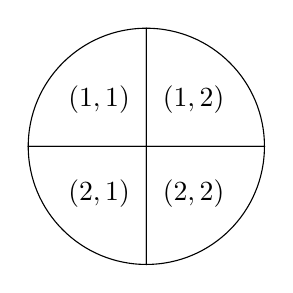
\begin{tikzpicture}
  % Define the fractions of the circle each segment occupies (in degrees)
  \newcommand{\A}{90}    % 20%
  \newcommand{\B}{90}   % 40%
  \newcommand{\C}{90}    % 20%
  \newcommand{\D}{90}    % 20%

  % Draw the segments
  \draw (0,0) -- (1.5,0) arc (0:\A:1.5) -- cycle;    % Segment A
  \draw(0,0) -- (\A:1.5) arc (\A:\A+\B:1.5) -- cycle; % Segment B
  \draw(0,0) -- (\A+\B:1.5) arc (\A+\B:\A+\B+\C:1.5) -- cycle; % Segment C
  \draw (0,0) -- (\A+\B+\C:1.5) arc (\A+\B+\C:\A+\B+\C+\D:1.5) -- cycle; % Segment D

  % Labels
  \node at (0.6,0.6) {$(1,2)$};
  \node at (-0.6, 0.6) {$(1,1)$};
  \node at (-0.6, -0.6) {$(2,1)$};
  \node at (0.6, -0.6) {$(2,2)$};
\end{tikzpicture}

\flushleft
For example, the above pie plot represents a basic principal stratification, whose $(S_i(1), S_i(2))$ are $(1,1), (1,2), (2,1), (2,2)$
\end{frame}

\begin{frame}{Examples for a principle stratification}
Example 1. Partition people into stratification where the treatment has no on $S$, i.e., $S_i(2) = S_i(1)$, i.e.,

Example 2. Partition people into stratification where $S_i(2)$ will always take 1 and 2, if the assigned treatment is $Z=2$.

    \begin{figure}[ht]
    \centering
    \begin{subfigure}{0.5\textwidth}
        \centering
        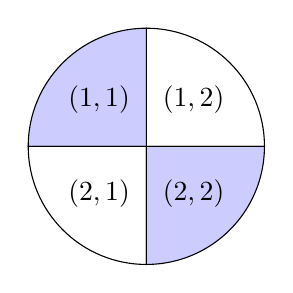
\begin{tikzpicture}
  % Define the fractions of the circle each segment occupies (in degrees)
  \newcommand{\A}{90}    % 20%
  \newcommand{\B}{90}   % 40%
  \newcommand{\C}{90}    % 20%
  \newcommand{\D}{90}    % 20%

  % Draw the segments
  \draw(0,0) -- (1.5,0) arc (0:\A:1.5) -- cycle;    % Segment A
  \draw[fill = blue!20](0,0) -- (\A:1.5) arc (\A:\A+\B:1.5) -- cycle; % Segment B
  \draw(0,0) -- (\A+\B:1.5) arc (\A+\B:\A+\B+\C:1.5) -- cycle; % Segment C
  \draw[fill = blue!20] (0,0) -- (\A+\B+\C:1.5) arc (\A+\B+\C:\A+\B+\C+\D:1.5) -- cycle; % Segment D

  % Labels
  \node at (0.6,0.6) {$(1,2)$};
  \node at (-0.6, 0.6) {$(1,1)$};
  \node at (-0.6, -0.6) {$(2,1)$};
  \node at (0.6, -0.6) {$(2,2)$};
\end{tikzpicture}
        \caption{Example 1: $S_i(1) = S_i(2)$}
        \label{fig:sub1}
    \end{subfigure}%
    \begin{subfigure}{0.5\textwidth}
        \centering
        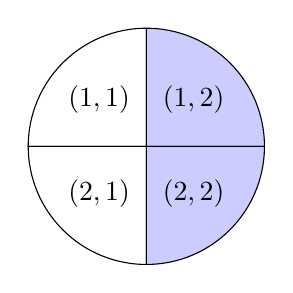
\begin{tikzpicture}
  % Define the fractions of the circle each segment occupies (in degrees)
  \newcommand{\A}{90}    % 20%
  \newcommand{\B}{90}   % 40%
  \newcommand{\C}{90}    % 20%
  \newcommand{\D}{90}    % 20%

  % Draw the segments
  \draw[fill = blue!20](0,0) -- (1.5,0) arc (0:\A:1.5) -- cycle;    % Segment A
  \draw(0,0) -- (\A:1.5) arc (\A:\A+\B:1.5) -- cycle; % Segment B
  \draw(0,0) -- (\A+\B:1.5) arc (\A+\B:\A+\B+\C:1.5) -- cycle; % Segment C
  \draw[fill = blue!20] (0,0) -- (\A+\B+\C:1.5) arc (\A+\B+\C:\A+\B+\C+\D:1.5) -- cycle; % Segment D

  % Labels
  \node at (0.6,0.6) {$(1,2)$};
  \node at (-0.6, 0.6) {$(1,1)$};
  \node at (-0.6, -0.6) {$(2,1)$};
  \node at (0.6, -0.6) {$(2,2)$};
\end{tikzpicture}
        \caption{Example 2: $S_i(2) = 1$ and $S_i(2) = 2$}
        \label{fig:sub2}
    \end{subfigure}
\end{figure}
\end{frame}

%---------------------------------------------------------
\begin{frame}{Principal effect w.r.t principal stratification}
\begin{block}{Definition}
Let $P$ be a principal stratification w.r.t. the posttreatment variable $S$ nd let $S_i^P$ indicate the stratum of $P$ to which unit $i$ belongs. Then a principal effect w.r.t. that principal stratification is defined as a comparison of potential outcomes under standard versus new treatment within a principal stratum $\varsigma$ in $P$, i.e., a comparison between the sets

\begin{equation}
\left\{Y_i(1): S_i^P=\varsigma\right\} \quad \text { and } \quad\left\{Y_i(2): S_i^P=\varsigma\right\}    
\end{equation}
\end{block}

Note that by definition, the values of $S_i(1), S_i(2)$ are affected by the treatment $Z$, which leads to 
\end{frame}

%---------------------------------------------------------
\begin{frame}{Properties}

\textbf{Property 1}: the stratum $S_i^P$ is unaffected by treatment for an principal stratifcation $P$.

\textbf{Property 2}: Any principal effect (2) is a causal effect because the comparison are on the same set of people.


\begin{itemize}
    \item Non-causal comparison
$$
\Pr\left\{Y_i(1) \mid S_i(1)=s\right\} \quad \text { and } \Pr\left\{Y_i(2) \mid S_i(2)=s\right\}
$$

\item Causal comparison

$$
\Pr\left\{Y_i(1) \mid S_i^P=\varsigma \right\} \quad \text { and } \Pr\left\{Y_i(2) \mid S_i^P=\varsigma \right\}
$$
\end{itemize}
\end{frame}

%---------------------------------------------------------
\begin{frame}{Inference based on the observed data}
Suppose we aim to estimate the principal effects, but have only observed data $H^{\text{obs}} = (Y^{\text{obs}}, S^{\text{obs}}, Z)$. There are two missing potential variables, $S^{\text{mis}} = \{S_i(z): \text{all}~ i; z \ne Z_i\}$ and $Y^{\text{mis}} = \{Y_i(z): \text{all}~ i; z \ne Z_i\}$. The observed likelihood is a marginal one that integrates over $(S^{\text{mis}}, Y^{\text{mis}})$


$$
\begin{aligned}
L& \left( H^{\mathrm{obs}} ; \theta^S, \theta^Y\right) \\
& = \iint \operatorname{pr}\left\{Z \mid(Y(1), Y(2)), S^{P_0}\right\}  \times \operatorname{pr}\left(S^{P_0} \mid \theta^S\right) \\
& \times \operatorname{pr}\left\{(Y(1), Y(2)) \mid S^{P_0} ; \theta^Y\right\} d Y^{\mathrm{mis}} d S^{\mathrm{mis}}
\end{aligned}
$$

where $\theta^Y, \theta^S$ represents the causal effect of $Z$ on $Y$ and $S$ respectively.

\end{frame}
%---------------------------------------------------------

\section{\S 4 Examples of Principal Effects in Action}

\begin{frame}{Three Examples}
Three important types of problems that can be handled through the 
framework of principal effects are 

\begin{itemize}
    \item[(i)] treatment noncompliance
    \item[(ii)] missing outcomes following treatment noncompliance, and 
    \item[(iii)] censoring by death. 
\end{itemize}
\end{frame}

%---------------------------------------------------------
\begin{frame}{Complier Average Causal Effect (CACE)}
Consider, for example, Imbens and Rubin's 
1997 re-analysis of data from a study on Vitamin A study where interest
was in the effect of \textbf{taking vitamin A vs. not taking vitamin A};
in other words, the causal effect when everyone assigned to 
treatment takes treatment and everyone assigned to nontreatment.

The CACE a special case of a principal effect:  this is a contrast 
of potential outcomes among the \textbf{"compliers"}, noting that "compliers" are a valid 
principal strata.

{\footnotesize *In general, regulatory agencies and practitioners do not 
trust the exchangeability assumptions necessary for uncontrolled compliance. 
\textit{Why would you approve a drug based on the effect of \underline{assignment}
to $Z=1$ or $Z=0$ when you could look at the actual effect?}}
\end{frame}

\begin{frame}{CACE Table}
From Imbens and Rubin 1997, \textit{Bayesian Inference for Causal Effects in Randomized Experiments with Noncompliance}:
\includegraphics[width=\textwidth]{figures/cace_figure/cace_table.png}

\scriptsize
\begin{itemize}
\item $D$ is the realized outcome (disease)
\item $C$ is the principal strata (complier, never-taker, always-taker, defier)
\item ITT = intention-to-treat
\item $Z$ is treatment
\item $Y$ is a potential outcome (inspired by Neyman's \textit{'potential yield'}) 
\item $Y(Z, \_)$ represents their potential outcome under assignment to treatment and what they did after. 
\end{itemize}
\normalsize

\end{frame}

%---------------------------------------------------------
\begin{frame}{Alternatives to CACE}
Note that the \textbf{CACE is a subgroup analysis}. It would be 
nice to use more of the data to estimate the complier-effect. 
However, other estimands require simulating what would have happened 
if, under some treatment level $Z=z$, 
\begin{enumerate}
    \item All subjects (including noncompliers) were somehow forced to take the 
    treatment; 
    \item All subjects (including noncompliers) would have been forced to take the control.
\end{enumerate}

\textbf{Simulating such scenarios poses issues}. Part of the problem 
arises from the fact that "forcing them" into treatment or nontreatment
is not a function of the controllable factor $Z$ alone, and therefore
the authors claim, does not lead to well-defined causal effects. 
\end{frame}

%---------------------------------------------------------
\begin{frame}{Missing Outcomes Following Treatment Noncompliance}
Consider the setting where \textbf{school-choice programs} are being evaluated through a
randomized intervention to provide school vouchers to children of low-income
parents. Posttreatment Problems:
\begin{enumerate}
    \item Actual use of the vouchers was uncontrolled; 
    \item Not every child took subsequent standardized tests (their choice of outcome) 
    to evaluate performance. 
\end{enumerate}

Frangakis and Rubin (1997, 1999) show that intention-to-treat analysis 
does not estimate intention-to-treat effects \textit{when there is 
outcome missingness dependent on post-treatment variables.}

The recommended, better approach is to use \textbf{principal strata} defined both by compliance and missingness. 
\end{frame}

%---------------------------------------------------------
\begin{frame}{Censoring Due to Death Dependent on Posttreatment}
Consider the time-ordered events: 

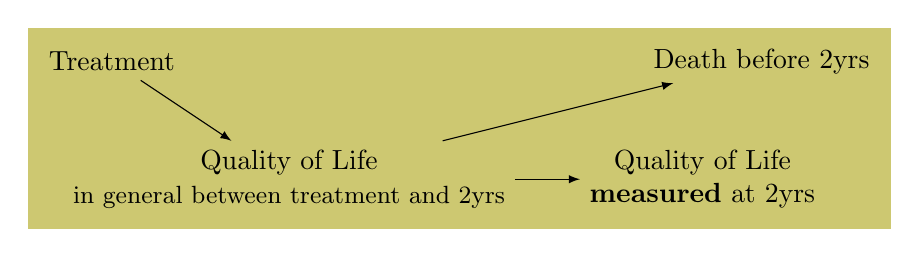
\begin{tikzpicture}[scale=3, background rectangle/.style={fill=olive!45}, show background rectangle]
\node (z) at (0,0) {Treatment};
\node (q1) [align=center] at (.75,-.5) {Quality of Life\\{\small in general between treatment and 2yrs}};
\node (q2) [align=center] at (2.5,-.5) {Quality of Life\\\textbf{measured} at 2yrs};
\node (d) at (2.75,0) {Death before 2yrs};

\draw[-latex] (z) -- (q1);
\draw[-latex] (q1) -- (q2);
\draw[-latex] (q1) -- (d);
\end{tikzpicture}

If QOL (Quality of Life at 2yrs) is censored due to death, we should not 
try to impute it because it's not a "missing value;" it's just a truly 
null value — a value that never existed in the first place. 

{\footnotesize Progress is made on the problem in Rubin's 2006 \textit{Causal Inference Through Potential
Outcomes and Principal Stratification: Application to Studies with ``Censoring"} 
by considering the principal stratification $\{$those who always live, 
those who always die, live under treatment + die under control, die under 
treatment + live under control$\}$. }

\end{frame}

%---------------------------------------------------------
\section{\S 5 Defining Surrogate Endpoints Using Causal Effects}

\subsection{5.1 Two Goals of Surrogate Endpoints and Previous Approaches}
\begin{frame}
\frametitle{Principle Stratum \& Surrogacy}
Define a randomized intervention $Z_i\in \{0,1\}$, mortality outcome $Y_i(z)$ as primary endpoint, and a surrogate variable for endpoint $S_i(z)$.\\
\vspace{1\baselineskip}
\begin{block}{Property of surrogacy}
\begin{enumerate}
	\item (Causal necessity): $Z$  has causal effect on $Y$ only if $Z$ has an effect on $S$.
	\item (Statistical generalizability):  $S^{obs}$ should be correlated with $Y^{obs}$ in application, even when $Y^{obs}$ is not immediately observed.
\end{enumerate}
\end{block}

\begin{itemize}
	\item Treatment can't act on outcome without manipulating surrogate.
	\item It's important to have predictability since observing mortality endpoint is unattainable.
\end{itemize}
\end{frame}

\begin{frame}
\frametitle{Principle Stratum \& Surrogacy}
Some past efforts to describe surrogacy:
\begin{itemize}
	\item ``$Y^{obs} = Y_i(Z=z_i)\ind Z_i \given S^{obs}_i$'' (Prentice 1989)
	\begin{itemize}
		\item Regression parameter coefficient, $R^2$, net treatment comparison
	\end{itemize}
\begin{definition}[\textsc{Traditional statistical surrogacy}]
\vspace{3mm}
$\displaystyle P\zuokh Y_i^{obs}\Big | Z_i=1,S^{obs}_i=s\youkh = P\zuokh Y_i^{obs}\Big | Z_i=2, S^{obs}_i=s\youkh$\\
\vspace{3mm}

\hfill  $\Longrightarrow$ $S$ is a \emph{statistical surrogate} for comparing effect of $Z$ on $Y$.
\end{definition}
\end{itemize}
\textcolor{red}{\bf Limitation}: Fail to satisfy the causal necessity property -- possible that unit whose treatment doesn't affect \emph{statistical surrogate} but affects outcome $\longrightarrow$ does not satisfy causal necessity.\\
\textcolor{teal}{\bf Solution}: Define an improved \emph{principal surrogate}.
\end{frame}

\subsection{5.2 Definition of Principle Surrogate and Property of Causal Necessity}

\begin{frame}
\small 
\frametitle{Principle Stratum \& Surrogacy}
\begin{definition}[\sc Principal surrogate]
\vspace{3mm}
$\displaystyle \{Y_i(1):S_i(1)=S_i(2)=s\}=\{Y_i(2):S_i(1)=S_i(2)=s\}, \forall \;s $\\
\vspace{3mm}
\hfill $\Longrightarrow$ $S$ is a principal surrogate for $Z$ and $Y$.
	
\end{definition}
Guarantees that causal effect of treatment on only exists when causal effect of treatment on surrogate exists (definition $\sim$ reads contrapositively).\\
\vspace{0.5\baselineskip}
Under randomization, principal surrogate implies:
$$
P\zuokh Y_i^{obs}\Big | Z_i=1,S_i(1)=S_i(2)=s\youkh = P\zuokh Y_i^{obs}\Big | Z_i=2, S_i(1)=S_i(2)=s\youkh
$$
and have corollaries: 
\begin{enumerate}
	\item $S$ is principal surrogate $\Longrightarrow$ $S$ is generally not a statistical surrogate;
	\item $S$ is statistical surrogate $\Longrightarrow$ $S$ is generally not a principal surrogate;
\end{enumerate}

Example with HIV treatment, CD4 counts, and mortality.
\end{frame}
%---------------------------------------------------------
\begin{frame}{\normalsize Figure 1a — Distinction between Principal and Statistical Surrogates}
\includegraphics[width=\linewidth]{figures/figure1/frangakis_rubin_figure.pdf}
{\footnotesize
Observe that if $S_i(1) = S_i(2) = s$, there is no effect of treatment
on the outcome. 
}
\end{frame}


%---------------------------------------------------------
\begin{frame}{\normalsize Figure 1b — Distinction between Principal and Statistical Surrogates}
\includegraphics[width=\linewidth]{figures/figure2/frangakis_rubin_figure2.pdf}
{\footnotesize
Controlling for a fixed level of $S_i^{obs} = s$, the observed treatment effect goes away. 
}
\end{frame}

\begin{frame}{Associative and Dissociative Effects}
Suggestion: Evaluate the effects of treatment on outcome that are 
associative and dissociative with effects on the posttreatment
variable. 

Treatment-outcome effects that are dissociative with effect on the surrogate are
comparisons between: 
$$\{ Y(1) : S(1) = S(2) \} \quad \text{ and } \quad \{ Y(0) : S(1) = S(2) \}.$$

On the other hand, treatment-outcome effects that are associative with effect
on the surrogate are comparisons between 
$$\{ Y(1) : S(1) \neq S(2) \} \quad \text{ and } \quad \{ Y(0) : S(1) \neq S(2) \}.$$
\footnotesize Large dissociative effect $\Rightarrow$ conclude large effect for 
subjects with CD4 unaffected. \newline 
\footnotesize Large associative effect $\Rightarrow$ conclude there is a 
large effect for subjects whose CD4 was affected by treatment.
\end{frame}


\subsection{5.3 Principal Stratification and Property of Statistical Generalizability}

%---------------------------------------------------------
\begin{frame}{Principal Stratification for Surrogate Endpoints: Setup}
Consider: How can principal stratification help us predict the outcomes 
in a randomized study that wants to use surrogate endpoints? E.g., 
to not wait for the expensive $Y^{\text{obs}}$. 

Let us consider the following probability models for a \underline{validation 
study $V$} and an \underline{application study $A$}: 

\begin{equation}
    P^V\{(S(1), S(2))\}, \quad P^V\{Y^{\text{obs}} | S(1), S(2), Z\}, \tag{V1} 
\end{equation}
\begin{equation}
    P^A\{(S(1), S(2))\}, \quad P^A\{Y^{\text{obs}} | S(1), S(2), Z\}. \tag{A1}
\end{equation}

Assume that all of the above are available except for $P^A(Y^\text{obs} | S(1), S(2), Z)$.
\end{frame}

\begin{frame}{Principal Stratification for Surrogates: \small Predictive Distribution\normalsize}
Before the outcomes $Y_i^\text{obs}$ are known in the application study, 
we can predict them according to the following distribution: 

$$P^A(Y^\text{obs} | S^{\text{obs}}, Z) = \frac{\int {\color{violet}{P^A\{Y^\text{obs} | S(1), S(2), Z \}}}
P^A \{ S(1), S(2)\} \mathrm d S^{\text{mis}}}{
\int P^A\{ S(1), S(2) \} \mathrm d S^{\text{mis}}}.
$$

However, this is not available to us because we do not have 
$\color{violet}{P^A(Y^\text{obs} | S(1), S(2), Z)}$.

*A common practice is to use $P^V(Y | S^\text{obs}, Z)$ but this replaces both
probability distributions of A1 with those of V1.
\end{frame}

\begin{frame}{Principal Stratification for Surrogates: Problem}
The \textit{\color{orange}problem} with this common practice is that the application 
study can differ from the validation study in either \textbf{distribution of principal strata}
or the \textbf{potential outcomes given the principal strata}.

This makes the predictive distribution incorrect for the application study. 

This could explain why the empirical distribution $P^V(Y^\text{obs} | S^\text{obs}, Z)$ 
may differ substantially from one validation study to another. 

Instead, consider that the right side of A1 matches the right 
side of V1 than it is that both sides match. 

$\Rightarrow$ Strategy: replace $P^A(Y^\text{obs}|S(1),S(2))$ with 
$P^{\color{red} V} (Y^\text{obs}|S(1), S(2))$
\end{frame}

\begin{frame}{Principal Stratification for Surrogates: Solution}
By replacing $P^A(Y^\text{obs}|S(1), S(2))$ with $P^{\color{red} V} (Y^\text{obs}|S(1), S(2))$, we obtain the synthetic predictive distrbiution: 
$$
P^\text{SYN}(Y^\text{obs}|S^\text{obs},Z) = 
\frac{\int P^V\{ Y^\text{obs}|S(1), S(2), Z \} P^A\{ S(1), S(2) \} \mathrm dS^\text{mis}}{
\int P^A\{ S(1), S(2) \} \mathrm dS^\text{mis} 
}.
$$

The authors claim that this should be a more plausible approximation
to the correct predictive distribution in the application study than 
just replacing ${\color{violet} P^A\{Y^\text{obs} | S(1), S(2), Z \}}$
with $P^V\{ Y^\text{obs} | S(1), S(2), Z \}$. 
\end{frame}

\begin{frame}
\footnotesize 
\frametitle{Estimation in Principal Stratification}
\framesubtitle{Likelihood function}
Recall unconfoundedness, $p( Z_i | Y_i(1), Y_i(0),D_i(1), D_i(0),X_i; \vec{\theta} )=p(Z_i|X_i)$ is the propensity score model,
\begin{align*}
	L(\vec{\theta })&=\prod^n_{i=1}p\zuokh Y_i(1), Y_i(0), D_i(0), D_i(1), Z_i,X_i; \vec{\theta} \youkh \\
	&= \prod^n_{i=1}\underbrace{p( Z_i | Y_i(1), Y_i(0),X_i; \vec{\theta} )}_{\text{const.}} \underbrace{p(  Y_i(1), Y_i(0)  |S_i, X_i; \vec{\theta}) }_{\text{unconfounded}}  p( S_i  | X_i; \vec{\theta})  p( X_i |\vec{\theta}) \\
	&\propto \prod^n_{i=1}\underbrace{p(  Y_i(1), Y_i(0)  |S_i, X_i; \vec{\theta})}_{outcome}   \underbrace{p( S_i  | X_i; \vec{\theta})}_{strata}  p( X_i |\vec{\theta})\\
	&\propto \prod_i p(Y_i(0)|S_i,X_i, \vec{\theta} )^{I(Z_i=0)}p(Y_i(1)|S_i,X_i, \vec{\theta} )^{I(Z_i=1)}p( S_i  | X_i; \vec{\theta})
\end{align*}
assuming potential outcome independence. Also  propensity score model is ignorable.
\end{frame}
         
\begin{frame}
\small  
\frametitle{Estimation in Principal Stratification}
\framesubtitle{Bayesian approach}
More granularly, individual stratum composition:
 $$
 L(\vec{\theta })\propto \prod^n_{i=1}\sum_{s\in S:D_i=D(s,Z_i)}p(S_i=s|X_i,\vec{\theta})p(Y_i|S_i=s,Z_i, X_i,\vec{\theta })
 $$
$S$ contains all possible strata; $D(s,z)$ is post-treatment variable under $s$ and treatment $z$ (Liu, 2023; Li, 2022). Resembles the form of a Gaussian mixture model: ``$\pi\mathcal{N}_1 + (1-\pi)\mathcal{N}_2$''.\\
\vspace{0.5\baselineskip}
Impose (multivariate) prior distribution $p(\vec{\theta})$ on parameter vectors that index two probability models, allowing us to harvest $p(\vec{\theta}|Z,D,Y,X)$, the posterior. \\
\vspace{0.5\baselineskip}
In reality,  compute posterior iteratively on: 1) $p(D^{mis}|Y^{obs},D^{obs}, Z,X;\theta)$ and 2) $p(\theta| Y^{obs},D^{mis,obs}, Z,X;\theta)$
\\
\vspace{0.5\baselineskip}
The \emph{principal causal effect} is identified as:
$$
PCE=\expect\zuo \expect[Y_i|Z_i=1,S_i=s,X_i]\given S_i=s\you-\expect\zuo \expect[Y_i|Z_i=2,S_i=s,X_i]\given S_i=s\you
$$
\end{frame}


\begin{frame}
\small 
\frametitle{Estimation in Principal Stratification}
\framesubtitle{Frequentist approach}
As a missing data (since all causality $\equiv$ missingness) \& specifically a latent mixture problem, \emph{EM algorithm} is also highly appropriate. \\
Same likelihood:
 $$
 L(\vec{\theta })\propto \prod^n_{i=1}\sum_{s\in S:D_i=D(s,Z_i)}p(S_i=s|X_i,\vec{\theta})p(Y_i|S_i=s,Z_i, X_i,\vec{\theta })
 $$
 \begin{itemize}
 	\item E-step: Impute $S_i^{t}$ with $\expect[S_i|Y^{obs}, D^{obs},X_i,\vec{\theta} ^t]$
 	\item M-step: Get gradient and optimize:
	$$
	\text{arg}\max_{\vec{\theta}}\; L(\vec{\theta}|Y^{obs}, S,X)
	$$
 \end{itemize}
\end{frame}




%---------------------------------------------------------
\section{\S 6 Remarks and Extensions} 

\begin{frame}{Authors' Remarks and Extensions}
For outcomes adjusted for posttreatment variables, we focused
on estimands before estimation by formulating principal causal effects. 

Basically any application of principal strata will require 
imputing missing information on the principal strata, i.e., 
the unobserved counterfactual of the post-treatment 
covariate under different treatment. 

Explicit restrictions such as latent ignorability* of outcome missingness or 
the compound exclusion restriction** can be 
more scientifically plausible than the implicit assumptions of 
standard approaches. 

A key contribution is formalizing what types of assumptions are needed for
estimating causal effects adjusted for post-treatment variables. 
\end{frame}

\begin{frame}{Authors' Remarks and Extensions: Necessary Footnotes}
\small
* As opposed to traditional ignorability assumptions 
that suppose conditioning on observed covariates, the potential outcomes
are independent of the treatment $Y(1), Y(2) \perp Z \mid L$, the 
latent ignorability assumption instead supposes that 
conditional on observed covariates and some possibly 
unobserved latent factors $U$, we have that $Y(1), Y(2) \perp Z \mid L, U$. 
\newline \newline 
One way this is written is $E[Y(1) | Z = 1, S = 1] = E[Y(1) | Z = 1, S = 0]$
and $E[Y(0) | Z = 0, S = 0] = E[Y(0) | Z = 1, S = 1]$. \newline

** The compound exclusion restriction 
is commonly seen in instrumental variables, and states that 
the instrumental variable $Z$ does not directly affect the outcome 
$Y$ except through the treatment and that there are no
unmeasured confounders of the $Z \sim Y$ relationship other than 
through the treatment. In this context, this means that 
the causal effect for the always-takers and never-takers is 
assumed to be 0. 
\normalsize
\end{frame}

\begin{frame}{Authors' Proposed Extensions}
Though we've considered the binary outcome and post-treatment variable case, the authors say 
the framework is immediately applicable to post-treatment variables that 
are multivariate, time-dependent, or continuous as well as continuous
treatments. 
\end{frame}

%---------------------------------------------------------
\begin{frame}{Authors' Summary}

\begin{block}{Summary} 
``Continued use of the current frameworks in problems with posttreatment
variables (e.g., surrogate endpoints) in principle makes \textcolor{orange!80!black!100}{\textbf{incorrect
attributions}} of effects of treatments.'' \newline \newline 'Until now, we had always thought that the roles of \textbf{biology 
and statistics did not mix} in these complex problems. But principal 
causal effects set the framework for allowing \textbf{biological assumptions} in statistical
methods and vice versa.' \newline \newline
``We hope that this article provokes the development and dissemination
of \emph{more principled frameworks}.''
\end{block}

\end{frame}

%---------------------------------------------------------
\section{Aftermath} 

\begin{frame}{Aftermath}
\begin{itemize}
    \item Very little practical recommendations \textit{in this paper} for how to estimate 
    $P(S(1), S(2))$; one of the key assumptions is that we have 
    access to $P(S(1), S(2))$. 
    \begin{itemize}
    \item {\footnotesize They highlight this in their statement 
    \textit{``we focused on estimands before estimation by formulating principal effects.''}}
    \item {\footnotesize }
    \end{itemize}
    \item Pearl 2011 (\textit{Transportability across studies: a formal approach}) heavily criticizes the idea of ``principal strata''
    \begin{itemize}
        \item {\footnotesize ``Their definition, called “principal surrogacy” requires
that causal effects of X on Y may exist if and only if causal effects of X on Z exist, ... but stops short of delineating the set of new
conditions under which this requirement should be sustained.''}
        \item {\footnotesize ``Rubin (2004) went further and proposed to do away with “deceptive” concepts such as direct and indirect
effects and replace them with “principal surrogacy.""}
    \end{itemize}
\end{itemize}
\end{frame}

\begin{frame}{Aftermath}
Mealli and Mattei respond in 2012 in Int. J. of Biostatistics: 

\footnotesize 
     A principal stratification with respect to a post-treatment variable is a partition 
     of units into latent classes defined by the joint potential values of that post-treatment variable under each of the treatments being compared. From this standpoint, some previous works (e.g., Robins (1986, 1998), Robins and Greenland
(1989a,b, 1994), [...], Heckman and Vytlacil (2001)), [...] can be viewed as 
examples of principal stratification. \ul{By definition,
principal strata are not affected by treatment assignment}, therefore a principal stratification 
can be used as any classification of units, to \textbf{define meaningful causal 
estimands} conditional on principal strata, to \textbf{discover treatment effect heterogeneities},
to \textbf{state identifying assumptions as behavioral assumptions on the principal strata}.

\tiny * Emphasis added
\normalsize
\end{frame}

%---------------------------------------------------------
\section*{Our Questions}

%---------------------------------------------------------
\section{Recommended References} 

\begin{frame}{Recommended References \hfill {\small (1/2)}}

\footnotesize
\begin{itemize}

\item Frangakis C. E., Rubin D. B. Principal stratification in causal inference. Biometrics. 2002 {\tiny \url{https://www.ncbi.nlm.nih.gov/pmc/articles/PMC4137767/}}


\item 
Zhang, J. L., \& Rubin, D. B. Estimation of Causal Effects via Principal Stratification When Some Outcomes Are Truncated by “Death.” Journal of Educational and Behavioral Statistics. 2003 28(4), 353–368. {\tiny \url{http://www.jstor.org/stable/3701340}}

\item 
Rubin, D. B. Causal Inference Through Potential Outcomes and Principal Stratification: Application to Studies with “Censoring” Due to Death. 2006 {\tiny \url{https://arxiv.org/abs/math/0612783}}

\item 
Imbens G. W., Rubin D.B. Annals of Statistics 1997. Bayesian Inference for Causal Effects in Randomized Experiments with 
Noncompliance. 
{\tiny \url{https://www.jstor.org/stable/2242722}}

\item 
Mealli F, Mattei A. A refreshing account of principal stratification. Int J Biostat (2012) {\tiny \url{https://pubmed.ncbi.nlm.nih.gov/22611592/}}

\item 
Grossi G, Mariani M, Mattei A, Mealli F. Bayesian principal stratification with longitudinal data and 
truncation by death (2023). {\tiny \url{https://arxiv.org/pdf/2401.00196.pdf}}

\end{itemize}

\normalsize
\end{frame}


\begin{frame}{Recommended References \hfill {\small (2/2)}}
\footnotesize 
\begin{itemize}
    \item Fan Li's Slides on Post-treatment Confounding: Principal Stratification {\tiny \url{http://www2.stat.duke.edu/\~fl35/teaching/640/Chapter6.2_principal\%20stratification.pdf}}

    \item Liu B., Li, F. \textsc{PStrata}: A package for Principal Stratification. Submitted to Journal of Statistical Software (2023) {\tiny \url{https://arxiv.org/abs/2304.02740}}

    \item Pearl, J. Principal stratification — A goal or a tool? {\tiny \url{https://ftp.cs.ucla.edu/pub/stat_ser/r382.pdf}}

    \item Tan X., Abberbock J., Rastogi P., Tang G. Identifying Principal Stratum Causal Effects Conditional on a Post-treatment 
    Intermediate Response. Proceeding of Machine Learning Research (2022) {\tiny \url{https://proceedings.mlr.press/v177/tan22a/tan22a.pdf}}

\end{itemize}
\normalsize
\end{frame}

%---------------------------------------------------------
\subsection*{Supplemental Materials}

\begin{frame}
Supplemental Materials
\end{frame}

\begin{frame}{Supplemental: Relationship to Mediation? \hfill {\small (1/2)}}
It's very natural to ask what is the relationship between 
this principal stratification framework and the framework of mediation?

{\small
See Mealli and Mattei (2012). The Principal Strata Direct Effect 
is the principal causal effect for the stratum where the intermediate 
variable $S(1) = S(2) = s$, i.e., $\mathrm{PSDE}(s) = E[Y(2) - Y(1) \mid S(1) = S(2) = s]$. 
Only in strata where the intermediate variable is unaffected by the treatment 
can we learn something about the direct effect of treatment. 

Causal mediation, on the other hand, focuses on disentangling 
direct and indirect effects. $\mathrm{NDE}(x) = E[Y(2, S(x)) - Y(1, S(x))]$, 
$\mathrm{NIE}(x) = E[Y(x, S(2)) - Y(x, S(1))]$, $x = 0, 1$ such that 
the average total causal effect $\mathrm{ATE} = \mathrm{NDE}(x) + \mathrm{NIE}(1-x)$. 

Conversely, principal stratification does not allow 
decomposition of the total effect into direct and indirect 
effects without additional assumptions.
}
\end{frame}

\begin{frame}{Supplemental: Relationship to Mediation? \hfill {\small (2/2)}}
Still from Mealli and Mattei (2012) (paraphrased): \newline \newline 
If $\mathrm{PSDE}(s) = 0$ for each $s \in \mathcal S$, then there is no evidence 
of direct effect of treatment after controlling for the mediator, because 
the causal effect only exists in the presence of an effect on the intermediate 
variable. 

This does not mean that there is no natural direct effect of the treatment: The principal causal 
effects for units in principal strata where post-treatment is affected by treatment 
('associative effects') combine natural direct and indirect effects. 
\end{frame}

\begin{frame}{Supplemental: Relationship to Instrumental Variables?}
Principal Stratification and Instrumental Variables are quite intrinsically linked in the 
sense that $Z$ (assignment to treatment) plays the role of an instrument and 
$S$ is actually taking the treatment. 

The assumption of monotonicity is saying there are no defiers, and the
exclusion-restriction is an assumption on the causal effects for 
always-takers and never-takers. 
\end{frame}

\begin{frame}{Supplemental: Approaches for Use in Practice}
\textsc{PStrata} implements a Bayesian approach (in Stan) for building $S$ and $Y$-models.

It appears to have been extended to interesting settings like longitudinal data, survival
analysis, multi-level data, etc.

{\footnotesize 
* That said, in theory, the approach can also be used with the EM-algorithm or
with a latent-mixture-modeling approach.
}
\end{frame}

\begin{frame}{Supplemental: What are the framework's limitations?}
\begin{itemize}
    \item Same criticisms as the Rubin Causal Model in general: is it okay to use unobservable counterfactuals?
    \begin{itemize}
        \item {\small However, if the post-treatment variables are not \textit{manipulable} we may not have the best  
        evidence to base counterfactuals where we assign treatment one way and post-treatment variables 
        another way (as if the unit had received a different level of treatment).}
    \end{itemize}
    \item You need a good model for the principal strata units fall into.
    \item Since the principal strata are never observable, you need strong identifying assumptions.
    \item May need a lot of data if there are lots of strata for which we need to estimate principal effects. 
\end{itemize}
\end{frame}

\begin{frame}{{\small Supplemental: \small Can you use IPW or DR with principal stratification?}}
There are some baseline considerations, like you can still have positivity violations just like in other settings.

But in general, we think one should be able to. 

\textsc{PStrata} claims to implement multiply-robust causal estimators under the 
principal stratification framework. 

{\small
Assuming principal ignorability, one can construct an inverse probability weighted 
multiply-robust estimator. 

The weighting based estimator is a produced of the inverse probability of 
three scores: the propensity score, principal score, and probability of the intermediate variable. 
If any of the two of the three models are correctly specified, then the 
estimator is consistent.

—from Liu and Li, 2023

\end{frame}

% \begin{frame}{{\small Supplemental: Can you validate a surrogate variable with principal stratification?}}
% In general, yes. Using principal stratification with an application and validation study, one can: 
% 
% \begin{itemize}
%     \item Assess models for the treatment on the candidate surrogate
%     \item Assess relationships between the candidate surrogate for the outcome
%     \item 
% \end{itemize}
% \end{frame}

\end{document}